\chapter{Impl\'ementation de la solution}

\section{Introduction}

Ce chapitre aborde comme sujet les choix technologiques et les outils pour l'impl\'ementation de notre solution ainsi que les captures d'\'ecran des diff\'erents fen\^etre r\'ealiser et les tests de validation effectu\'es sur les modules d\'evelopp\'es.

\section{Environnement logiciel}
L'environnement logiciel utilis\'e pour la r\'ealisation de notre projet est pr\'esent\'e dans le tableau suivant :

\begin{table}[H]
\begin{center}
\begin{tabularx}{\textwidth}{ |l|X| }
\hline Outil & Description \\\hline \hline
JDK 1.8 & Java Development Kit (JDK) d\'esigne un ensemble de biblioth\`eques logicielles de base du langage de programmation Java.\\ \hline
Intellij IDEA & Environnement de d\'eveloppement int\'egr\'e (IDE).\\ \hline
Visual Studio Code & Environnement de d\'eveloppement c\^ote frontend.\\ \hline
Android Studio & Environnement de d\'eveloppement pour d\'evelopper des applications mobiles Android.\\ \hline
GitBash & C'est une ligne de commande dans laquelle on peut ex\'ecuter les commandes git.\\ \hline
Zeplin & C'est un outil de design des fonctionnalit\'es. Permet de collaborer entre les designers et les d\'eveloppeurs frontends, facile, efficace et permet de gagner du temps.\\ \hline
Postman & Est actuellement l'un des outils les plus populaires utilis\'es dans les tests d'\gls{API}.\\
\hline
\end{tabularx}
\caption{Environnement logiciel}
\end{center}
\end{table}

\section{Architecture technique du syst\`eme}

Notre syst\`eme se base en totalit\'e sur l'architecture orient\'e service et plus pr\'ecis\'ement sur l'architecture \gls{REST}. C'est un style d'architecture pour la conception d'applications faiblement coupl\'ees sur \gls{HTTP}, souvent utilis\'e dans le d\'eveloppement de services Web.

Une \'etude qui a \'et\'e faite par l'entit\'e \gls{DF}, ils sont convaincu d'adapter quelques technologies qu'on va les utiliser. La figure suivante repr\'esente les technologies utilises dans notre projet.

\begin{figure}[H]
	\center{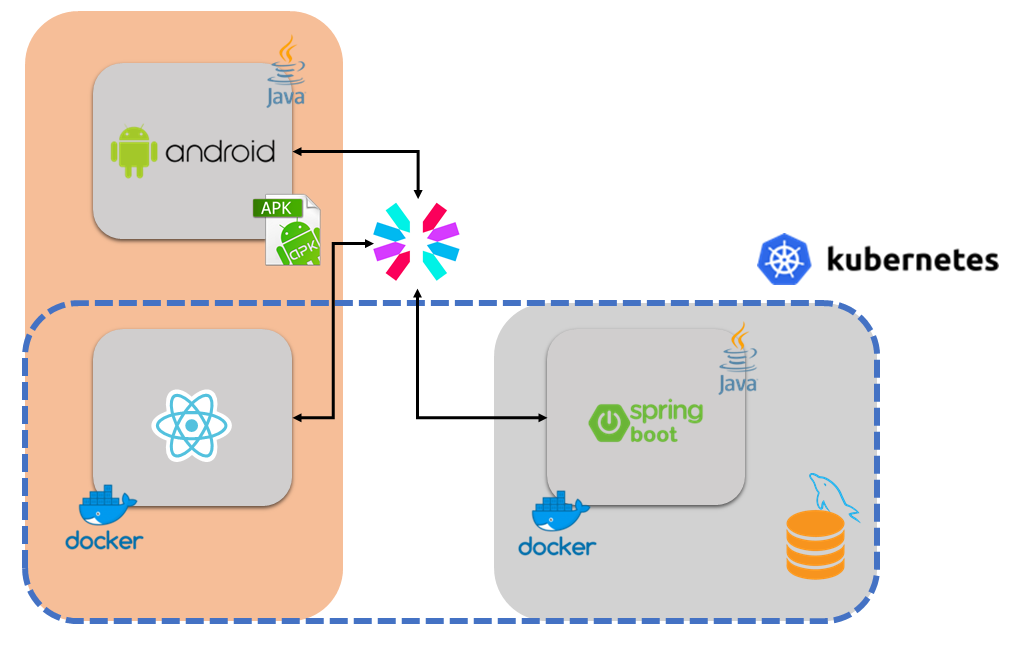
\includegraphics[width=\textwidth]{Figures/achitec-tech.PNG}}
	\caption{\label{fig:my-label} Architecture technique du syst\`eme}
\end{figure}

Maintenant, on va expliquer l'utilit\'e des technologies utilises dans notre impl\'ementation. 

\subsection{Couche BackEnd}
\begin{itemize}

\item \textcolor{spring}{SpringBoot} : est un framework Java open source utilis\'e pour cr\'eer un Micro Service. Il est d\'evelopp\'e par l'\'equipe \textbf{pivotal}. Il est facile de cr\'eer des stand-alone applications. Spring Boot contient une prise en charge compl\`ete de l'infrastructure pour le d\'eveloppement d'un micro-service et vous permet de d\'evelopper des applications d'entreprise.

\item \textbf{Spring Security} : est un Framework de s\'ecurit\'e l\'eger qui fournit une authentification et un support d'autorisation afin de s\'ecuriser les applications Spring. Il est livr\'e avec des impl\'ementations d'algorithmes de s\'ecurit\'e populaires.

\item \textbf{Swagger} : nous permet de d\'ecrire la structure de nos API afin que les machines puissent les lire. La capacit\'e des API \`a d\'ecrire leur propre structure facilite aux d\'eveloppeurs frontend la communication avec nos serveurs.

\item \gls{JWT} : est une normalisation permettant d'utiliser des jetons pour s'authentifier sur le Web en g\'en\'eral. Il est robuste et peut contenir beaucoup d'informations. Comme tout autre jeton, JWT peut \^etre utilis\'e pour transmettre l'identit\'e d'utilisateurs authentifi\'es entre un fournisseur d'identit\'e et un fournisseur de services. Il peut \'egalement contenir toutes les revendications de l'utilisateur, telles que les donn\'ees d'autorisation. Le fournisseur de services n'a donc pas besoin d'entrer dans la base de donn\'ees ou dans des syst\`emes externes pour v\'erifier les r\^oles et autorisations des utilisateurs pour chaque demande. Ces donn\'ees sont extraites du jeton.

\end{itemize}

\subsection{Couche FrontOffice}
\begin{itemize}

\item \textcolor{react}{ReactJS} : est essentiellement une biblioth\`eque JavaScript open-source qui est utilis\'ee pour cr\'eer des interfaces utilisateur sp\'ecifiquement pour les applications à page unique. React nous permet \'egalement de cr\'eer des composants d'interface utilisateur r\'eutilisables.

\item \textcolor{redux}{Redux} : Biblioth\`eque compl\'ementaire \`a React qui permet de conserver facilement les donn\'ees (State) et les \'ev\'enements (Actions) .Redux isole l'objet d'\'etat des composants.

\item \textbf{Redux-saga} : est une biblioth\`eque de middleware redux con\c{c}ue pour simplifier la gestion des effets secondaires de votre application redux. Pour ce faire, il exploite une fonctionnalit\'e de l'ES6 appel\'ee Generators, qui nous permet d'\'ecrire un code asynchrone qui a l'air synchrone et qui est tr\`es facile \`a tester.

\end{itemize}

\subsection{Couche BackOffice}
\begin{itemize}

\item

\end{itemize}
